% Revisão bibliográfica
%
% Fundamentação teórica do trabalho. Aqui deve ser revisto tudo o que
% foi utilizado para a concepção do trabalho.

\subsection{Caldeiras aquatubulates}

\begin{figure}[H]
\caption{\label{fig_circulo} Esquema de uma caldeira aquatubular}
\begin{center}
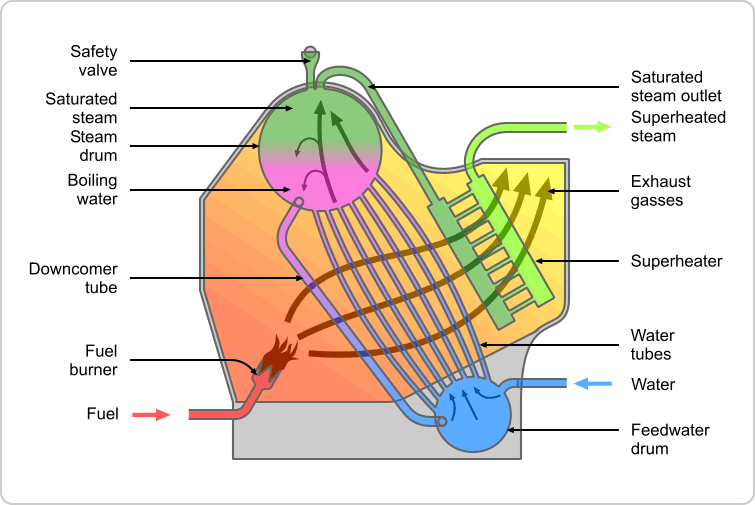
\includegraphics[scale=0.75]{img/caldeira.png}
\end{center}
\legend{Fonte: \citeonline{wikiwatertube}}
\end{figure}

O que diferencia uma caldeira aquatubular das outras é a localização
da água e do sistema de combustão: a água fica dentro de tubos,
enquanto a combustão ocorre fora dos tubos. Também pode-se dizer que o
material dos tubos sofre forças de tensão, uma vez que a pressão é
gerada internamente \cite{boilers}. Um esquema simplificado da
caldeira pode ser visto na figura \ref{fig_circulo}.

\subsubsection{Funcionamento}
Na caldeira aquatubular, existem dois tubulões ligados por dois
conjuntos de tubos: ascendentes e descendentes. Um dos tubulões fica
em baixo, alimentado por uma entrada de água. O tubulão superior é
preenchido até um certo nível por água, sendo o restante preenchido
por vapor. No tubulão superior o vapor é coletado, normalmente
passando por um superaquecedor para diminuir a umidade do vapor que
alimentará a planta.

O calor é transferido para a água através dos tubos ascendentes. Por
causa do aquecimento direto dos tubos, uma diferença entre a densidade
da água no tubo ascendente e o tubo descendente faz com que ocorra uma
circulação de água natural entre os tubos. Dessa forma, a água
aquecida sobe pelos tubos ascendentes, libera o vapor no tubulão
superior e então retorna para o tubulão inferior através dos tubos
descendentes \cite{ufrj}. Para caldeiras de maior pressão, as
densidades da água nos tubos ascendentes e descendentes começam a
assumir valores próximos, impossibilitando a circulação natural da
água. Nessas caldeiras, bombas hidráulicas são acionadas e circulam a
água na caldeira.

Para se controlar o nível do tubulão, atua-se na válvula de entrada de
água, ou seja, alterando a vazão de entrada de água. A
diferença entre a vazão de entrada e a vazão de saída (na forma de
vapor) proporciona o aumento ou diminuição do nível de água no tubulão
superior, ao alterar a quantidade total de água no sistema. Isso pode
ser visto na equação a seguir:


\begin{equation}
  \dfrac{d}{dt} (\rho_s V_{st} + \rho_w V_{wt}) = q_f - q_s
  \label{balanco_global_massa}
\end{equation}

Aqui, os subscritos $s$ e $w$ se referem ao vapor e água,
respectivamente. $\rho$ e $q$ são, respectivamente, densidades
e vazões mássicas. $V_{st}$ e $V_{wt}$ são os volumes de vapor e água
dentro da caldeira.


Esse volume total de água influencia diretamente o nível de água no
tubulão, porém não é a única variável. Efeitos de dilatação e
contração devidos à mudanças na pressão e na temperatura também
influenciam o nível, o que faz o controle do mesmo ser uma tarefa
complicada \cite{astrom}. Em \citeonline{astrom} é desenvolvido um
modelo matemático dinâmico com o intuito de representar essa variação
do nível em caldeiras de grande porte e circulação natural de
água. A construção desse modelo é apresentada a seguir.

\subsection{Modelo matemático}

A maior parte do comportamento dinâmico do sistema pode ser descrito
através dos balanços de massa e energia globais do sistema. A equação
\ref{balanco_global_massa} é o balanço global de massa, enquanto a equação do
balanço global de energia pode ser escrita como:

\begin{equation}
  \dfrac{d}{dt} (\rho_s u_s V_{st} + \rho_w u_w V_{wt} + m_t C_p t_m)
  = Q + q_f h_f - q_s h_s
  \label{balanco_global_energia0}
\end{equation}

O lado direito da equação \ref{balanco_global_energia0} mostra o fluxo
de energia que é recebido através do calor proveniente da queima do
combustível, somado à energia interna da água de alimentação ($ Q +
q_f h_f $). Também mostra o fluxo de energia entregue pela caldeira
através do vapor ($q_s h_s$).

Onde $h$ é entalpia, $u$ é energia interna, $m_t$ é a massa total de
metal dos tubos, $C_p$ é o calor específico do metal e $t_m$ é a
temperatura do mesmo. \citeonline{astrom} diz que o sistema pode ser
considerado sempre termicamente em equilíbrio, ou seja, considera-se a
temperatura do metal igual à temperatura de saturação do vapor
($t_s$), que é função da pressão $p$ da caldeira.

A equação a seguir relaciona os volumes de água e vapor com o volume
total da caldeira ($V_t$):
\begin{equation}
  V_t=V_{wt}+V_{st}
  \label{vol_total}
\end{equation}

A energia interna de um sistema pode ser representada como $u = h - p
/ \rho$, onde $p$ é a pressão interna da caldeira. Utilizando a
equação \ref{vol_total} e a relação da energia interna, pode-se
reescrever a equação \ref{balanco_global_energia0} da seguinte forma:

\begin{equation}
  \dfrac{d}{dt} (\rho_s h_s V_{st} + \rho_w h_w V_{wt} - p V_t + m_t C_p t_m)
  = Q + q_f h_f - q_s h_s
  \label{balanco_global_energia}
\end{equation}

Em uma caldeira, as variáveis $Q$, $q_f$ e $q_s$ podem ser mensuradas
direta ou indiretamente. $q_s$ depende da demanda da planta, enquanto
$Q$ é controlado por malhas externas ao controle de nível. A variável
$q_f$ é usada como variável de controle, uma vez que o sistema atua na
válvula de entrada de água para o controle de nível. A saída do
sistema será sua pressão ($p$) e o nível da água no tubulão superior
($l$).

$\rho_w$, $\rho_s$, $h_w$, $h_s$, e $t_s$ são propriedades
térmodinâmicas da água. Por estarem a temperatura próxima da
temperatura de saturação, pode-se representá-las como função somente
da pressão \cite{garland}. Já as propriedades termodinâmicas da água
de alimentação, por esta estar a uma baixa temperatura em relação ao
sistema, podem ser consideradas funções somente da temperatura
\cite{garland2}.

Por enquanto as equações \ref{balanco_global_massa} e
\ref{balanco_global_energia} conseguem descrever o comportamento da
pressão e da quantidade de água total com relação a alterações no
calor e vazões de entrada de água e saída de vapor, mas não descreve o
comportamento do nível de água, uma vez que, por serem equações de
balanços globais, não apresentam informações sobre a distribuição do
vapor no interior do tubulão. É a forma de distribuição do vapor e da
água no interior da caldeira que dá origem aos efeitos de contração
e expansão, uma vez que o vapor pode estar localizado abaixo do nível
da água na forma de pequenas bolhas, o que caracteriza um sistema de
escoamento bifásico.

Sistemas de escoamento bifásico são normalmente modelados usando
equações diferenciais parciais e elementos finitos, mas um modelo
simplificado do mesmo é suficiente para a simulação da caldeira.

Esse modelo pode ser encontrado usando os balanços de massa e energia
no tubo ascendente. As equações são, respectivamente:

\begin{equation}
  A\dfrac{\partial \rho} {\partial t} + \dfrac{\partial q}{\partial z}
  = 0
  \label{balanco_massa_riser}
\end{equation}

\begin{equation}
  \dfrac{\partial \rho h}{\partial t} + \dfrac{1}{A} \dfrac{\partial q
    h}{\partial z} = \dfrac{Q}{V}
  \label{balanco_energia_riser}
\end{equation}

No caso, as variáveis são:
\begin{itemize}
\item[$ \rho $]: Densidade da mistura de água e vapor
\item[$ t $]: Tempo
\item[$ q $]: Vazão mássica da mistura
\item[$ h $]: Entalpia da mistura
\item[$ A $]: Área de uma seção transversal
\item[$ V $]: Volume do tubo
\item[$ Q $]: Calor entregue ao tubo
\end{itemize}

\begin{figure}[H]
  \caption{\label{riser} Esquema simplificado das variáveis dinâmicas
    do tubo ascendente}
  \begin{center}
    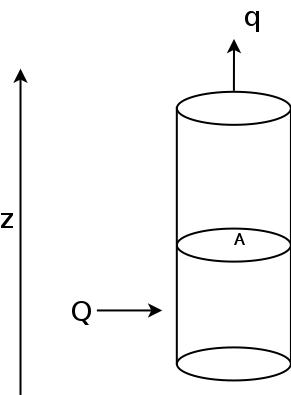
\includegraphics[scale=0.3]{img/riser.png}
  \end{center}
\end{figure}

Para simplificar o modelo, foi considerado que a variação das
variáveis com relação aos eixos $X$ e $Y$ é nula, portanto todas as
variáveis do sistema são funções de $z$ e $t$.

Então, se $\alpha_m$ é definida como a fração do fluxo mássico
constituída de vapor, tem-se a seguinte equação:

\begin{equation}
  h=\alpha_m h_s + (1-\alpha_m) h_w = h_w + \alpha_m h_c
  \label{entalpia_mist_riser}
\end{equation}


Em regime permanente, as seguintes igualdades são derivadas das
equações \ref{balanco_massa_riser} e \ref{balanco_energia_riser}:

\begin{equation}
  \dfrac{\partial q}{\partial z} = 0
  \label{balanco_massa_riser_rp}
\end{equation}

\begin{equation}
  \dfrac{1}{A} \dfrac{\partial q h}{\partial z} = \dfrac{Q}{V}
  \label{balanco_energia_riser_rp}
\end{equation}


Substituindo as equações \ref{balanco_massa_riser_rp} e
\ref{balanco_energia_riser_rp} na equação \ref{entalpia_mist_riser},
tem-se:

\begin{equation}
  \alpha_m = \dfrac{Q A}{q h_c V} z
  \label{eq_alfa_m}
\end{equation}

Para facilitar os cálculos, define-se a variável $\xi$ como o
comprimento normalizado do tubo ascendente, ou seja, se $ L $ é o
comprimento total do tubo e $L_i$ um comprimento qualquer, tem-se
$\xi=L_i / L$. Logo, $0 \leq \xi \leq 1$.

Define-se a qualidade do vapor que sai em um ponto do tubo ascendente 
como $\alpha_r$, relacionando-se com $\alpha_m$ da seguinte maneira:

\begin{equation}
  \alpha_m(\xi)=\alpha_r\xi
  \label{alpha_r_m_lin}
\end{equation}

Na realidade, existe um escorregamento entre o vapor e a água que
causa uma não linearidade na relação entre $\alpha_m$ e $\alpha_r$,
porém de acordo com dados experimentais o escorregamento pode ser
ignorado \cite{astrom}.

A fração volumétrica também é uma função da fração mássica, definida
da seguinte forma:

\begin{equation}
  \alpha_v=\dfrac{ \rho_w \alpha_ m}{ \rho_s + (\rho_w - \rho_s) *
    \alpha_m } 
  \label{alpha_v_alpha_m}
\end{equation}

Essa modelagem, apesar de utilizar o modelo linear para o cálculo de
$\alpha_m$, mostrou-se próxima dos dados reais, como mostra o gráfico
da figura \ref{alpha_v_pde_lin}.

\begin{figure}[H]
  \caption{\label{alpha_v_pde_lin} Comparação entre resultados em
    regime permanente do modelo simplificado de $\alpha_v$ e
    resolução de equações diferenciais parciais}
  \begin{center}
    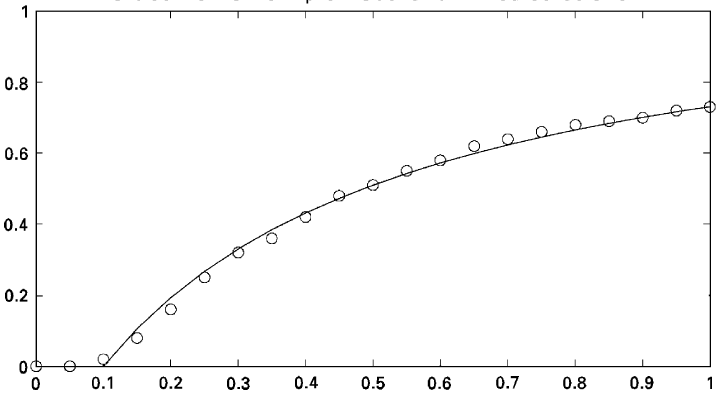
\includegraphics[scale=0.25]{img/alpha_v_pde_lin.png}
  \end{center}
  \legend{Fonte: \cite{astrom}. A linha contínua representa o modelo
    simplificado (equações \ref{alpha_r_m_lin} e
    \ref{alpha_v_alpha_m}), enquanto os círculos representam soluções
    numéricas a partir de equações diferenciais parciais complexas. }
\end{figure}

Para encontrar o nível de água, é necessário encontrar o volume total
de vapor nos tubos ascendentes. Para isso, é necessário encontrar a
fração volumétrica média ($ \bar{\alpha_v} $) nos tubos:

\begin{center}
  $\bar{\alpha}_v = \dfrac{1}{\alpha_m(1)} \int_0^{\alpha_m(1)}
  \alpha_v(\alpha_m) d\alpha_m $
\end{center}

A partir da equação \ref{alpha_r_m_lin}, pode-se perceber que
$\alpha_m(1) = \alpha_r$ e $d\alpha_m = \alpha_r d\xi$. Logo

\begin{center}
  $\bar{\alpha}_v = \dfrac{1}{\alpha_r} \int_0^{\alpha_r}
  \alpha_v(\xi) \alpha_r d\xi$
\end{center}

\begin{equation}
  \bar{\alpha}_v = \dfrac{\rho_w}{\rho_w - \rho_s}
  \biggl( 1 - \dfrac{\rho_s}{(\rho_w - \rho_s)\alpha_r} ln\biggl( 1 +
  \dfrac{\rho_w - \rho_s}{\rho_s} \alpha_r \biggr) \biggr)
  \label{alfa_v_avg}
\end{equation}

Outro elemento importante para a simulação é a transferência de massa
e energia entre o vapor e a água através da condensação e
evaporação. Para evitar a necessidade de contabilizar explicitamente
tal transferência, as equações de balanço energético e mássico da água
e vapor são escritas em conjunto, sendo o balanço global de massa nos
tubos ascendentes representado por

\begin{equation}
  \dfrac{d}{dt} (\rho_s \bar{\alpha}_v V_r + \rho_w (1 -
  \bar{\alpha}_v)V_r) = q_{dc} - q_r
  \label{balanco_massa_riser}
\end{equation}

Onde $q_r$ e $q_{dc}$ são, respectivamente, os fluxos mássicos saindo
e entrando do tubo ascendente.

O balanço global de energia no tubo ascendente é

\begin{equation}
  \dfrac{d}{dt} (\rho_s h_s \bar{\alpha}_v V_r + \rho_w h_w (1 -
  \bar{\alpha}_v)V_r - pV_r + m_r C_p t_s) = Q + q_{dc} h_w -
  (\alpha_r h_c + h_w) q_r
  \label{balanco_energia_riser}
\end{equation}

Onde $h_c$ é a entalpia de condensação:

\begin{equation}
  h_c = h_s - h_w
  \label{h_c}
\end{equation}

As equações \ref{balanco_massa_riser} e \ref{balanco_energia_riser}
presumem a linearidade da relação explicitada através da equação
\ref{alpha_r_m_lin} mesmo fora do regime permanente, anulando a
necessidade de usar equações diferenciais parciais.

Em caldeiras de recirculação natural, o valor de $q_{dc}$ é governado
pelos gradientes de densidade nos tubos ascendente e descendente. Esse
balanço de momento pode ser demonstrado por

\begin{equation}
  (L_r + L_{dc}) \dfrac{d q_{dc}}{dt} = (\rho_w - \rho_s)
  \bar{\alpha}_v V_r g - \dfrac{k q_{dc}^2}{2 \rho_w A_{dc}}
  \label{balanco_momento_recirculacao}
\end{equation}

Onde $L_r$ e $L_{dc}$ são os comprimentos dos tubos ascendentes e
descendentes e $A_{dc}$ é a área da seção transversal do tubo
descendente.

Pode-se perceber que a equação \ref{balanco_momento_recirculacao}
representa um sistema de primeira ordem, onde sua constante de tempo é

\begin{center}
$ T = \dfrac{(L_r + L_{dc}) A_{dc} \rho_w}{k q_{dc}} $
\end{center}
  
\citeonline{astrom} calcula que para valores típicos de caldeiras
reais, essa constante gira em torno de $1s$ e, como o período de
amostragem é cerca de dez vezes maior ($10s$), pode-se dizer que o
sistema da equação \ref{balanco_momento_recirculacao} é rapido o
suficiente para legitimar a utilização da relação em regime
permanente, como mostra a equação a seguir.

\begin{equation}
  \dfrac{1}{2} k q_{dc}^2 = \rho_w A_{dc} (\rho_w - \rho_s) g
  \bar{\alpha}_v V_r
  \label{q_dc}
\end{equation}

Apesar da geometria complicada e arranjos complexos encontrados nas
caldeiras, pode-se representar o comportamento da distribuição de
vapor no tubulão através dos mecanismos básicos de separação de água e
vapor e de condensação. Tem-se que o balanço de massa de vapor abaixo
do nível de água líquida é:

\begin{equation}
  \dfrac{d}{dt} (\rho_s V_{sd}) = \alpha_r q_r - q_{sd} - q_{cd}
  \label{balanco_massa_s_abaixo_nivel}
\end{equation}

Onde $V_{sd}$ é o volume de vapor abaixo do nível de líquido e
$q_{sd}$ é a vazão mássica de vapor através da superfície do
líquido. $q_{cd}$ é a vazão de condensação no tubulão, definida por:

\begin{equation}
  q_{cd} = \dfrac{h_w - h_f}{h_c} q_f + \dfrac{1}{h_c} \biggl( \rho_s
  V_{sd} \dfrac{dh_s}{dt} + \rho_w V_{wd} \dfrac{dh_w}{dt} - (V_{sd} +
  V_{wd}) \dfrac{dp}{dt} + m_d C_p \dfrac{dt_s}{dt} \biggr)
  \label{q_cd}
\end{equation}

Onde $V_{wd}$ é o volume de água líquida abaixo do nível de líquido.

A vazão mássica de vapor através da superfície da água é comandada
pela diferença de densidade entre a água e o vapor, e em
\citeonline{astrom} foi desenvolvido o seguinte modelo empírico para
representá-lo:

\begin{equation}
  q_{sd} = \dfrac{\rho_s}{T_d}(V_{sd} - V_{sd}^0) + \alpha_r q_{dc} +
  \alpha_r \beta (q_{dc} - q_r)
  \label{q_sd}
\end{equation}

Onde $V_{sd}^0$ é o volume de vapor no tubulão em uma situação
hipotética em que não á condensação de vapor, $T_d$ é o tempo de
permanência do vapor no tubulão e $\beta$ é uma constante empírica.

Com isso, pode-se representar o volume de água na caldeira:

\begin{equation}
  V_{wd} = V_{wt} - V_{dc} - (1 - \bar{\alpha}_v) V_r
  \label{V_wd}
\end{equation}

Como o tubulão tem uma geometria complicada, usa-se um modelo
linearizado descrito pela superfície molhada ($A_d$) no ponto de
operação. A variável $l$ será então a variação do nível medida a
partir do ponto de operação normal. Essa variação é representada por

\begin{equation}
  l = \dfrac{\dfrac{V_{wd} + V_{sd}}{A_d} - l_o}{l_o}
  \label{nivel_agua}
\end{equation}

Onde as contribuições do vapor e da água no nível total são,
respectivamente

\begin{equation}
  l_w = \dfrac{\dfrac{V_{wd}}{A_d} - l_{wo}}{l_{wo}}
  \label{contrib_w_nivel}
\end{equation}

\begin{equation}
  l_s = \dfrac{\dfrac{V_{sd}}{A_d} - l_{so}}{l_{so}}
  \label{contrib_s_nivel}
\end{equation}

Onde $l_o$, $l_{wo}$ e $l_{so}$ são os valores dos níveis e
contribuições no ponto de operação da caldeira. Em
\citeonline{astrom}, tais valores foram omitidos das equações de $l$,
$l_w$ e $l_s$, mas contabilizados na apresentação dos resultados.

Usando-se das equações apresentadas, pode-se construir um sistema
da seguinte forma:

\begin{equation}
  E(X) \times \dot{X} = U
  \label{sistema_geral}
\end{equation}

Onde $X$ é o vetor de estado, $U$ o vetor de entrada e $E(X)$ uma
matriz de variáveis dependentes das variáveis de estado, com os
seguintes valores.

\begin{equation}
  X = \begin{bmatrix}
    V_{wt} \\
    p \\
    \alpha_r \\
    V_{sd}
  \end{bmatrix}
  \label{X_vec}
\end{equation}

\begin{equation}
  U = \begin{bmatrix}
    q_f - q_s \\
    Q + q_fh_f - q_s h_s \\
    Q - \alpha_r h_c q_{dc} \\
    \dfrac{\rho_s}{T_d} (V_{sd}^0 - V_{sd}) + \dfrac{h_f - h_w}{h_c}
    q_f
    \end{bmatrix}
  \label{U_vec}
\end{equation}

Pode-se perceber através dos valores de $X$ e $U$ que as variáveis de
estado são $V_{wt}$, $p$, $\alpha_r$ e $V_{sd}$, enquanto as variáveis
de entrada são $q_f$, $q_s$ e $Q$.

\begin{equation}
  E(X) = \begin{bmatrix}
    e_{11} & e_{12} & 0 & 0 \\
    e_{21} & e_{22} & 0 & 0 \\
    0 & e_{32} & e_{33} & 0 \\
    0 & e_{42} & e_{43} & e_{44} \\
  \end{bmatrix}
  \label{E_x_mat}
\end{equation}

Onde:

\begin{equation}
  \begin{cases}
    e_{11} = \rho_w - \rho_s \\
    e_{12} = V_{wt} \dfrac{\partial \rho_w}{\partial p} + V_{st}
    \dfrac{\partial \rho_s}{\partial p} \\
    e_{21} = \rho_w h_w - \rho_s h_s \\
    e_{22} = V_{wt} \biggl(h_w \dfrac{\partial \rho_w}{\partial p} +
    \rho_w \dfrac{\partial h_w}{\partial p}\biggr) + V_{st} \biggl(h_s
    \dfrac{\partial \rho_s}{\partial p} + \rho_s \dfrac{\partial
      h_S}{\partial p}\biggr) - V_t + m_t C_p \dfrac{\partial
      t_s}{\partial p} \\
    e_{32} = \biggl(\rho_w \dfrac{\partial h_w}{\partial p} - \alpha_r
    h_c \dfrac{\partial \rho_w}{\partial p} \biggr) (1 - \bar{\alpha}_v)
    V_r + \biggl( (1-\alpha_r) h_c \dfrac{\partial \rho_s}{\partial p} 
    + \rho_s \dfrac{\partial h_s}{\partial p} \biggr) \bar{\alpha}_v V_r \\
    +  (\rho_s + (\rho_w - \rho_s)\alpha_r) h_c V_r \dfrac{\partial 
      \bar{\alpha}_v}{\partial p} - V_r + m_r C_p \dfrac{\partial
    t_s}{\partial p} \\
    e_{33} = ((1 - \alpha_r)\rho_s + \alpha_r \rho_w) h_c V_r
    \dfrac{\partial \bar{\alpha}_v}{\partial \alpha_r}\\
    e_{42} = V_{sd} \dfrac{\partial \rho_s}{\partial p} + \dfrac{1}{h_c}
    \biggl(\rho_s V_{sd} \dfrac{\partial h_s}{\partial p} + \rho_w
    V_{wd} \dfrac{\partial h_w}{\partial p} - V_{sd} - V_{wd} + m_d C_p
    \dfrac{\partial t_s}{\partial p}\biggr) + \alpha_r (1 + \beta) V_r\\
    e_{43} = \alpha_r (1 + \beta)(\rho_s - \rho_w)V_r \dfrac{\partial \bar{\alpha}_v}{\partial \alpha_r}\\
    e_{44} = \rho_s
  \end{cases}
  \label{eij_vals}
\end{equation}

Derivando a equação \ref{alfa_v_avg} obtém-se

\begin{equation}
  \begin{cases}
    \dfrac{\partial \bar{\alpha}_v}{\partial p} = \dfrac{1}{(\rho_w -
      \rho_s)^2} \biggl(\rho_w \dfrac{\partial \rho_s}{\partial p} -
    \rho_s\dfrac{\partial \rho_w}{\partial p} \biggr) \biggl(1 +
    \dfrac{\rho_w}{\rho_s} \dfrac{1}{1+\eta} - \dfrac{\rho_s +
      \rho_w}{\eta \rho_s} \ln(1+\eta)\biggr) \\
    \dfrac{\partial \bar{\alpha}_v}{\partial \alpha_r} =
    \dfrac{\rho_w}{\rho_s \eta} \biggl(\dfrac{1}{\eta} \ln(1+\eta) -
    \dfrac{1}{1 + \eta}\biggr)
  \end{cases}
  \label{derivs_alfa_v_avg}
\end{equation}

Onde $\eta = \alpha_r (\rho_w - \rho_s)/\rho_s$.

Com o modelo apresentado, pode-se encontrar as variações de $X$ em
função do tempo, ou seja, basta ter uma estimativa dos parâmetros
iniciais e o simulador pode funcionar.

Para encontrar condições iniciais, pode-se usar a solução da equação
\ref{sistema_geral} em regime permanente:

\begin{equation}
  \begin{cases}
    q_f = q_s \\
    Q = q_s h_s - q_f h_f \\
    Q = q_{dc} \alpha_r h_c \\
    V_{sd} = V_{sd}^0 - \dfrac{T_d(h_w-h_f)}{\rho_s h_c} q_f
  \end{cases}
  \label{sistema_geral_rp}
\end{equation}

Escolhe-se inicialmente um valor para $q_s$ e, a partir desse valor,
encontra-se $q_f$. $q_{dc}$ pode ser encontrado também usando a
equação \ref{q_dc} em regime permanente e então encontra-se $Q$. Com o
valor de $Q$, usa-se a seguinte equação,  juntamente com a equação
\ref{alfa_v_avg} para a criação de um sistema de equações não linear.

\begin{equation}
  Q=\alpha_r h_c \sqrt{\dfrac{2 \rho_w A_{dc} (\rho_w - \rho_s) g
      \bar{\alpha}_v V_r}{k}} 
  \label{Q_lin_sys}
\end{equation}

A resolução desse sistema resulta no valor de $\alpha_r$. Basta
substituir os valores calculados na última equação do sistema para
encontrar $V_{sd}$

Com o valor de $\dot{X}(t)$, pode-se calcular facilmente $X(t_i)$
realizando a integração numérica de $ \int_0^{t_i} \dot{X}(t) dt $.
  
De acordo com \citeonline{astrom}, o modelo apresentado necessita
somente dos seguintes parâmetros da planta real:

\begin{itemize}
\item Volume do tubulão ($ V_d $)
\item $ V_r $
\item $ V_{dc} $
\item $ A_d $
\item $ m_t $
\item $ m_r $
\item $ k $
\item $ T_d $
\item $ \beta $
\end{itemize}

Porém, como visto pelo desenvolvimento do modelo, os seguintes
parâmetros também devem ser estimados:

\begin{itemize}
\item Temperatura da água de entrada ($ t_f $)
\item $ A_{dc} $
\item $ V_{sd}^0 $
\item $l_o$
\end{itemize}

Há ainda algumas equações e variáveis secundárias, úteis para a
validação da simulação. São elas:

Vazão de condensação em toda a caldeira ($q_{ct}$):

\begin{equation}
  q_{ct} = \dfrac{h_w - h_f}{h_c} q_f + \dfrac{1}{h_c} \biggl( \rho_s
  V_{st} \dfrac{dh_s}{dt} + \rho_w V_{wt} \dfrac{dh_w}{dt} - V_t
  \dfrac{dp}{dt} + m_t C_p \dfrac{dt_s}{dt} \biggr)
  \label{q_ct}
\end{equation}


\subsection{Controle de nível}

Em uma caldeira aquatubular, o controle de nível é feito atuando-se na
válvula de entrada de água na caldeira, ou seja, a atuação é feita na
variável $q_f$.

O controle de nível usado nesse trabalho visa eliminar os problemas
causados por variações na pressão da água de alimentação, sendo mais
eficiente por ter uma resposta mais rápida e com menos oscilação
\cite{ufrj}. Para isso, usa-se três variáveis da caldeira: vazão do
vapor, nível de água do tubulão e vazão da água de entrada. Cada um
dos três elementos pertence a uma submalha do sistema, formando um
sistema de controle em cascata em que o nível de água do tubulão é a
saída. A malha está representada na figura \ref{malha_3_elementos}.

\begin{figure}[H]
  \caption{\label{malha_3_elementos} Malha de controle de nível
  a três elementos}
  \begin{center}
    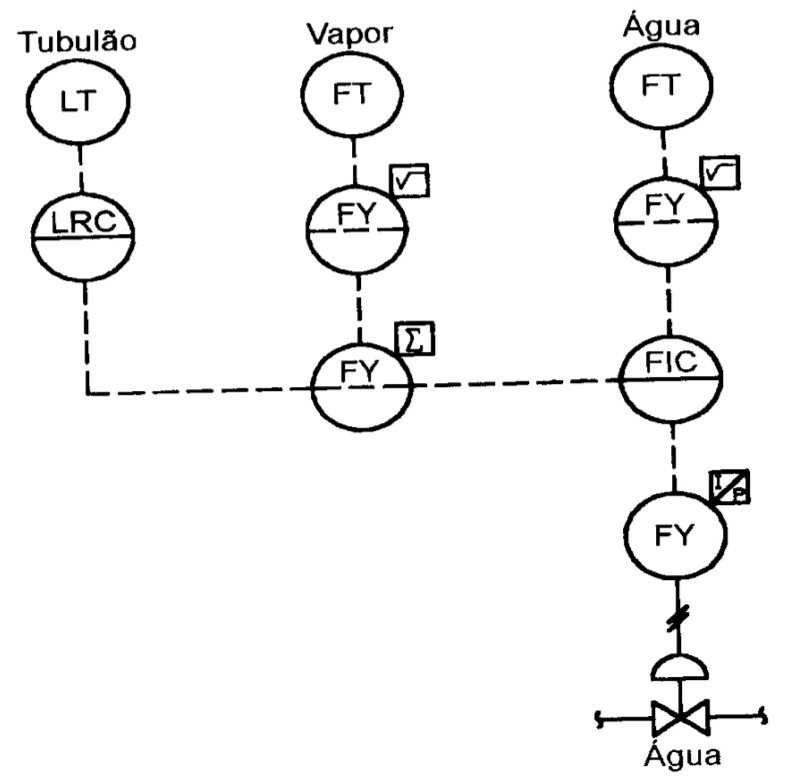
\includegraphics[scale=.35]{img/malha_3_eltos.png}
  \end{center}
  \legend{Fonte: \citeonline{ufrj}}
\end{figure}

As seguintes siglas são utilizadas (legenda retirada de
\citeonline{isa-1984}):

\begin{itemize}
\item \textbf{LT} (transmissor de nível): Captura o nível do tubulão e
  transmite para uma unidade de processamento;
\item \textbf{FT} (transmissor de vazão): Captura a vazão e transmite
  para uma unidade de processamento;
\item \textbf{LRC} (controlador de nível): Recebe o sinal de nível e
  gera um sinal de controle na saída;
\item \textbf{FY} (dispositivo de cálculo): Realiza cálculos baseados
  na entrada e sua função. As seguintes funções foram usadas na
  malha:
  \begin{itemize}
  \item Para o símbolo $\sqrt{\phantom{x}}$, calcula-se $Y=\sqrt{X}$;
  \item Para o símbolo $\Sigma$, calcula-se $Y=\sum_{i} X_i$;
  \item para o símbolo $^I/_P$, o bloco transforma o sinal de corrente
    em um sinal pneumático;
  \end{itemize}
  Onde $X$ é a entrada e $Y$ a saída no bloco;
\item \textbf{FIC} (controlador de vazão): Com base nos sinais de
  entrada, gera um sinal de controle a ser aplicado na válvula de saída
\end{itemize}

No caso, o FIC e o FY com símbolo $^I/_p$ estão contidos no modelo da
válvula de controle de vazão de entrada de água. Teoricamente,
portanto, seriam necessários modelos de válvulas tanto para a entrada
de água quanto para a saída de vapor. Um bom modelo seria capaz de
mostrar as perdas de pressão e o comportamento dinâmico da vazão
durante o acionamento da válvula.

\subsection{Controle de pressão}

Em caldeiras de vapor, normalmente a pressão é mantida em torno de um
valor constante, capaz de suportar a carga máxima para a qual a
caldeira foi projetada \cite{brantly1942steam}. Esse controle da
pressão é feito através da alteração do fluxo de calor entregue à
caldeira: para se aumentar a pressão, basta aumentar o fluxo de calor
entregue. Como demonstrado em \cite{controle-pressao}, um controle
proporcional-integral é suficiente para tal.

\begin{figure}[htb]
  \caption{\label{blocospressao} Diagrama de blocos do controle de
    pressão de uma caldeira}
  \begin{center}
    \begin{tikzpicture}[auto, node distance=2cm,>=latex']
        % We start by placing the blocks
        \node [input, name=input] {};
        \node [sum, right of=input] (sum) {};
        \node [block, right of=sum] (controller) {PI};
        \node [block, right of=controller, node distance=3.2cm] (queimador) {Queimador};
        \node [block, right of=queimador, node distance=3.2cm]
        (caldeira) {Caldeira};
        \node [output, right of=caldeira] (output) {};
        \coordinate [below of=controller] (tmp);
            
        % Once the nodes are placed, connecting them is easy.
        \draw [draw,->] (input) -- node {$p_u$} (sum);
        \draw [->] (sum) -- node {$e$} (controller);
        \draw [->] (controller) -- node {$Q_u$} (queimador);
        \draw [->] (queimador) --node {$Q$} (caldeira);
        \draw [->] (caldeira) --node [name=out] {$p$} (output);
        \draw [->] (out) |- (tmp) -| node[pos=.99] {$-$} (sum);
    \end{tikzpicture}
  \end{center}
\end{figure}


\subsection{Trocas de mensagens entre processos}

Em arquiteturas de software distribuídas, a troca de informações entre
os processos é essencial. Essa troca de informações usa protocolos de
comunicação comuns e é chamada de \textit{comunicação inter-processos}
\cite{wikiipc}. Os processos podem estar na mesma máquina física ou em
localidades separadas, podendo usar vários protocolos diferentes para
a comunicação, desde TCP/IP até pipes de sistemas POSIX.

Tendo a comunicação inter-processo em mente, o sistema de filas de
mensagens (\textit{Message Queueing System}, abreviado por
\textit{MQ}) é usado. Um MQ é um sistema que disponibiliza uma
interface aos processos para que os mesmos possam trocar mensagens
entre si \cite{feldbaum2002method}. Esse sistema é gerenciado por um
processo externo e várias implementações disponibilizam serviços como
balanceamento de carga, ordenação das mensagens (por prioridade ou
FIFO, por exemplo) e mecanismos de segurança para troca de mensagens.

\subsubsection{Padrões de mensagens}
Padrões de mensagens são a forma com que o os nós da comunicação irão
consumir e gerar mensagens, sendo cada padrão adequado a um problema
\cite{zmq}. Para o trabalho proposto, apenas dois dos padrões
disponíveis foram utilizados. Ambos estão explicados nas seções a
seguir.

\subsubsubsection{Padrão request-reply}

O padrão request-reply é o padrão mais simples. Nele, existe um
servidor e um cliente, de tal forma que o segundo envia mensagens de
requisição ao primeiro. Ao receber uma requisição, o servidor responde
com outra mensagem. Um servidor pode receber mensagem de vários
clientes, mas um cliente só envia mensagem para um servidor por vez.

\subsubsubsection{Padrão push-pull}

No padrão push-pull não há entidades cliente-servidor. Ao invés disso,
existe o produtor e o consumidor, onde o produtor envia mensagens ao
consumidor. O consumidor não irá responder, mas pode continuar
enviando o resultado do processamento da mensagem recebida ao próximo
consumidor do fluxo, tornando-se o produtor da nova relação. Pode
existir uma associação de vários produtores enviando mensagens para um
consumidor ou vários consumidores recebendo mensagem de um único
produtor.
